
\chapter{Introduction}

	One of the main topics in computer vision is object recognition. Despite many years of research that brought us all kinds of artificial algorithms, very basic problems remain nearly unsolvable.
	
	An example would be this simple decision task: Is there a bird in an image? Humans can answer this after seeing a picture for only very short duration although they never saw the image before. More surprisingly it also does not matter if a person knows that exact type of bird or if he had seen it before. Viewing positions and angles, photometric effects, scene settings and changing body shapes have little effect on the overall test performance.
	
	It is obvious this is the product of a long evolutionary process that lead to a high efficient object recognition system like the one in humans. So if it works this well, the naive solution is to design new algorithms the same way the human visual system works.
	
	To gain an understanding of what these new models should achieve, we are starting to look at the physiology in chapter 2. After covering the anatomy of the retina and the information transport to the brain, the complexity of the visual cortex will be addressed.
	
	Chapter 3 starts off with some background about what kind of model will be used. The basis for all of them will be the results of \citeauthor{hubel1962receptive}'s research that is shortly explained and then used to implement the HMAX model by \citeauthor{riesenhuber1999hierarchical}. \citeauthor{serre2007robust} refined this model and also discussed the biological plausibility. To emphasize the performance of the developed models this chapter concludes with a comparison to artificial state-of-the-art algorithms.
	
	As the main task of this seminar is to find a biological inspired way for self-localization, chapter 4 comes back to that and links the acquired models to that application. It is basically object recognition but with some boundary conditions and many additional work.
	
	
\chapter{Human Visual System}

	Until today the human vision is the best-known system for recognizing objects and actions in a scene is a very short time. The basis to understand how it works lies in the anatomy and physiology. Therefore all the parts that belong to the visual cortex are described here.
	
	\section{Retina}
		
		The retina is the only source for visual stimuli in mammals. This is an excellent prerequisite to study neural responses, because all input can easily be controlled.
		
		Figure \ref{retina-cross-section} shows a cross section through a human eye. Light enters through the lens that (ideally) focuses a sharp image onto the foeva. The foeva is the part of the retina with the highest density of cells and is the area with which humans most consciously see. The photons travel through all layers before getting absorbed and transfered into neuronal signals at the photo receptors.
		
		\begin{figure}[H]
			\centering
			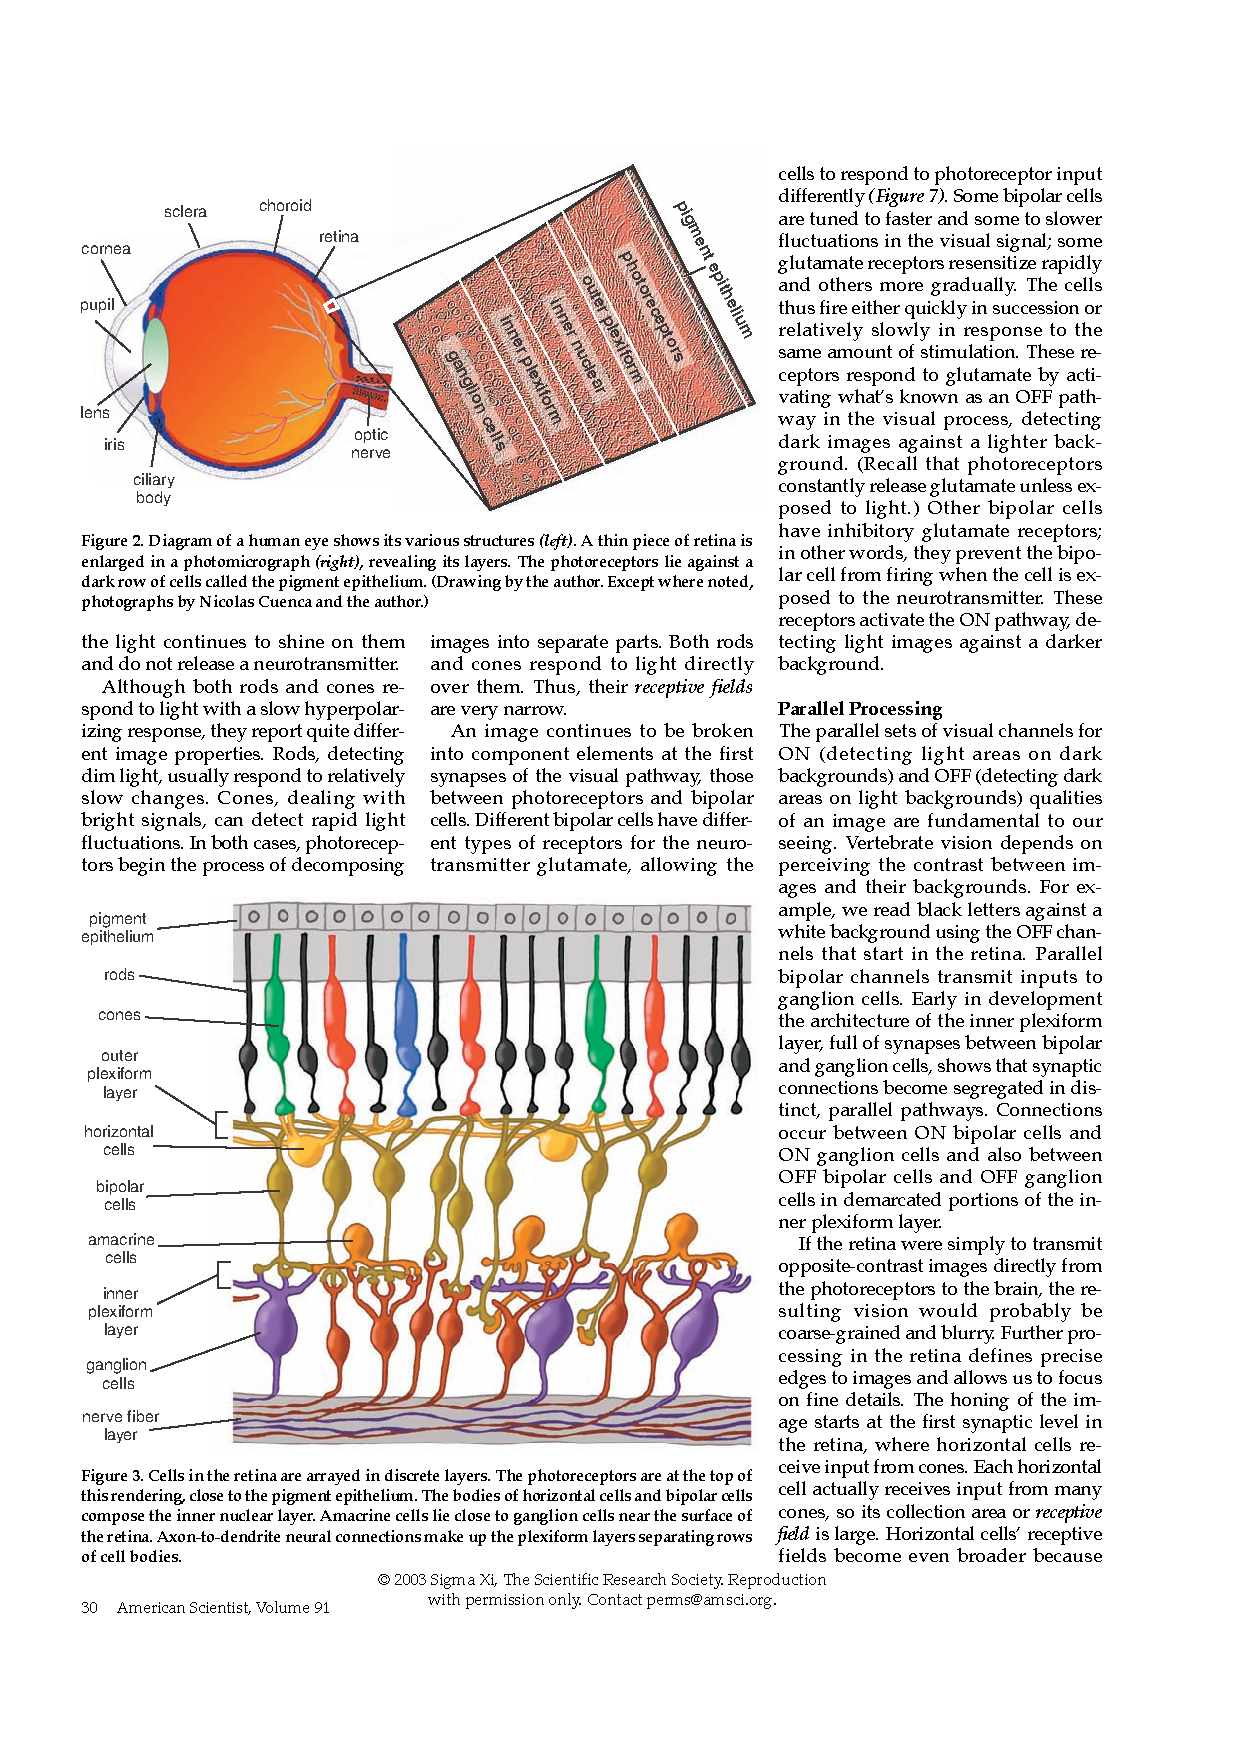
\includegraphics[width=0.8\textwidth, trim=1cm 21cm 8cm 2.5cm, clip]{images/kolb-2003-howtheretinaworks-p3.pdf}
			\caption{Cross section of the human eye \citep{kolb2003retina}}
			\label{retina-cross-section}
		\end{figure}
		
		There is already processing happening in the layers of the retina before the information goes on the optic nerve. The photo receptive cells, the rods and cones, generate an analog signal in the outer plexiform layer. This is the input of the bipolar cells that transport the signal to the inner plexiform layer. With interaction between bipolar and horizontal cells, the visual system is able to adapt to different illuminations. In the inner plexiform layer the dentrites of ganglion cells and amacrines combine the data from different bipolar cells before it get converted to action potentials and sent out of the retina.
		
		Overall the information is encoded into a string of about 1 million ganglion axons that are called the optic nerve. It transports the information to the optic chiasm.
		
		\begin{figure}[H]
			\centering
			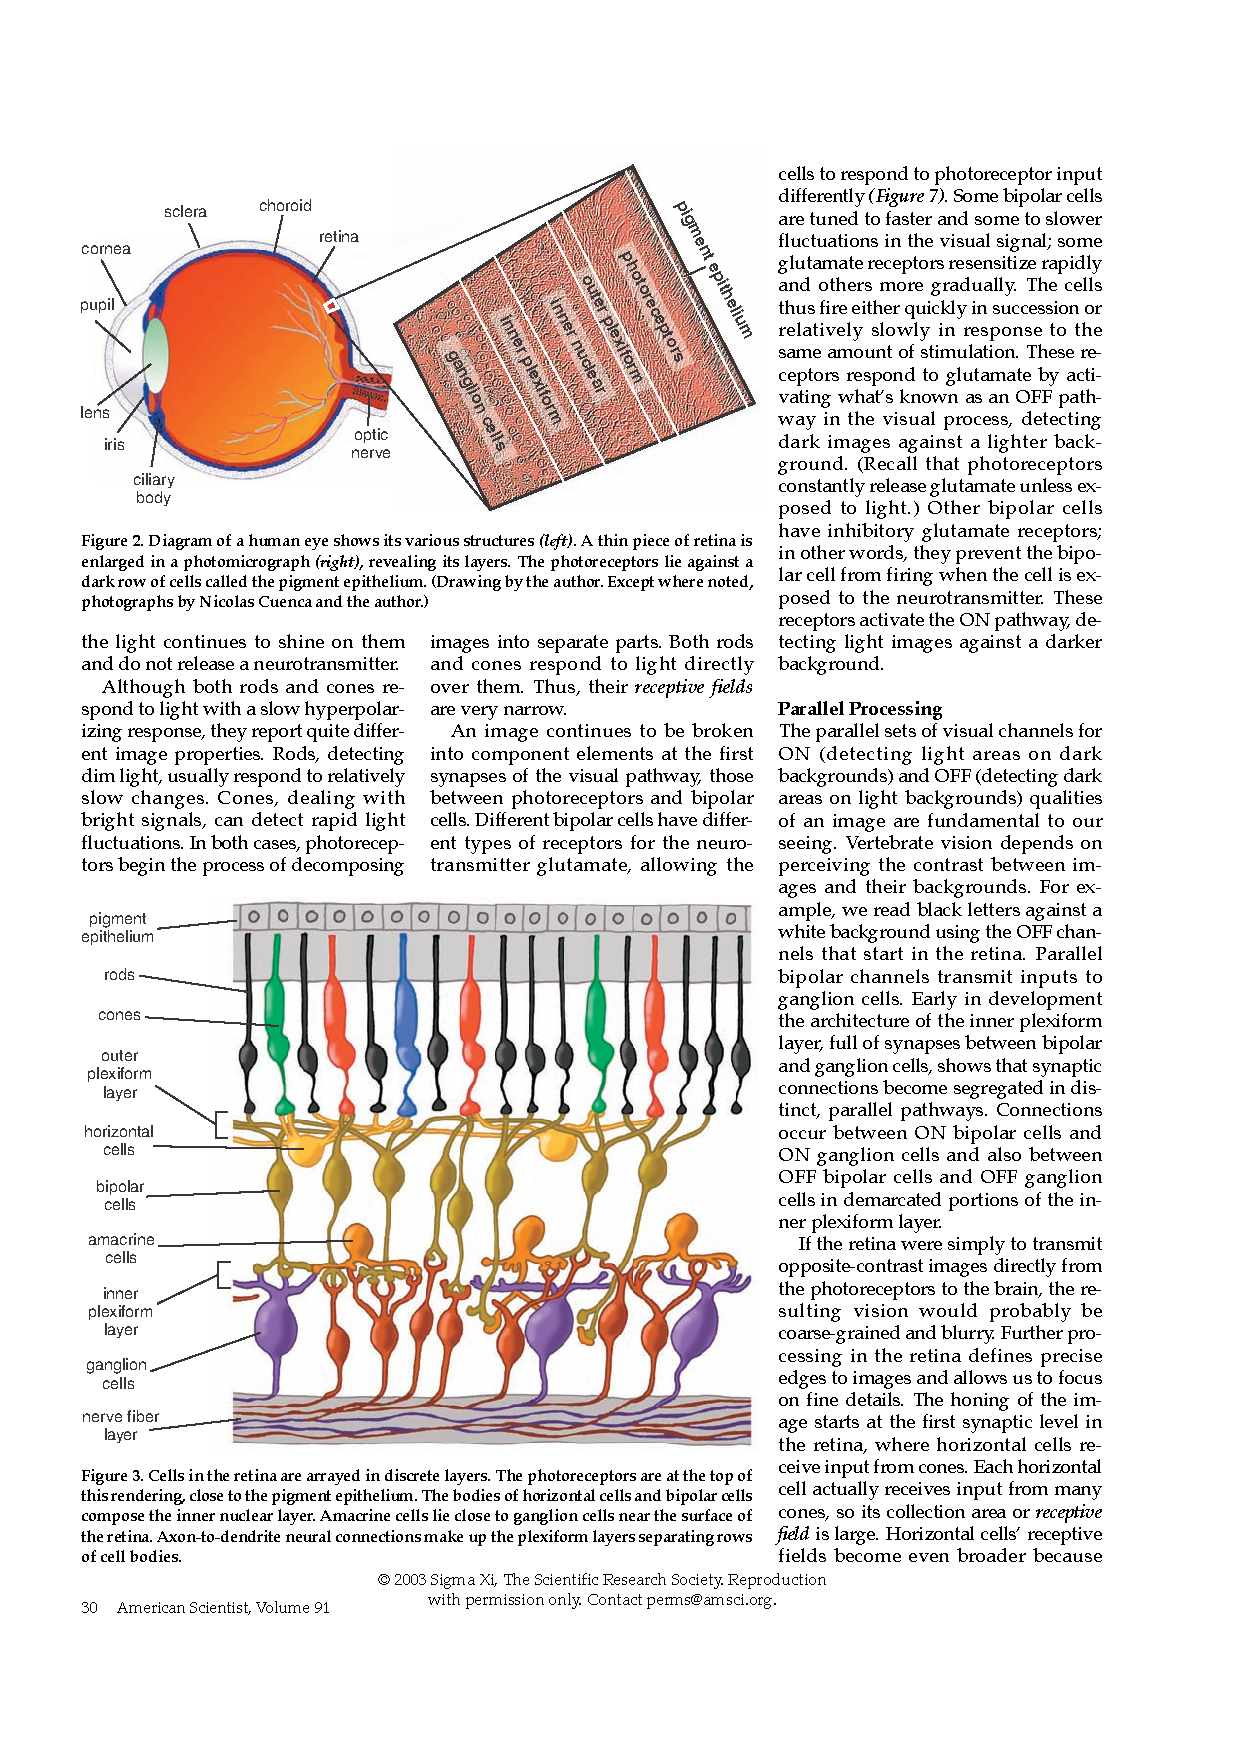
\includegraphics[width=0.8\textwidth, trim=1cm 5cm 8cm 15cm, clip]{images/kolb-2003-howtheretinaworks-p3.pdf}
			\caption{Cross section of the retina \citep{kolb2003retina}}
		\end{figure}
		
		So what is the output of the retina? Ganglion cells are connected to many rods and cones each but their specific function differs drastically. Mostly there are cells that fire when the center of their receptive field is illuminated and the surroundings are not, or the other way around (OFF- and ON-center cells).
		
		Additionally there are ganglion cells that are responsible for special low level functions. For example the focusing of the eye or the signal inhibition when the eye of head moves and would overflow the cortex with information (object motion sensitive cells).
		
		\begin{figure}[H]
			\centering
			\captionsetup{justification=centering,margin=0.5cm}
			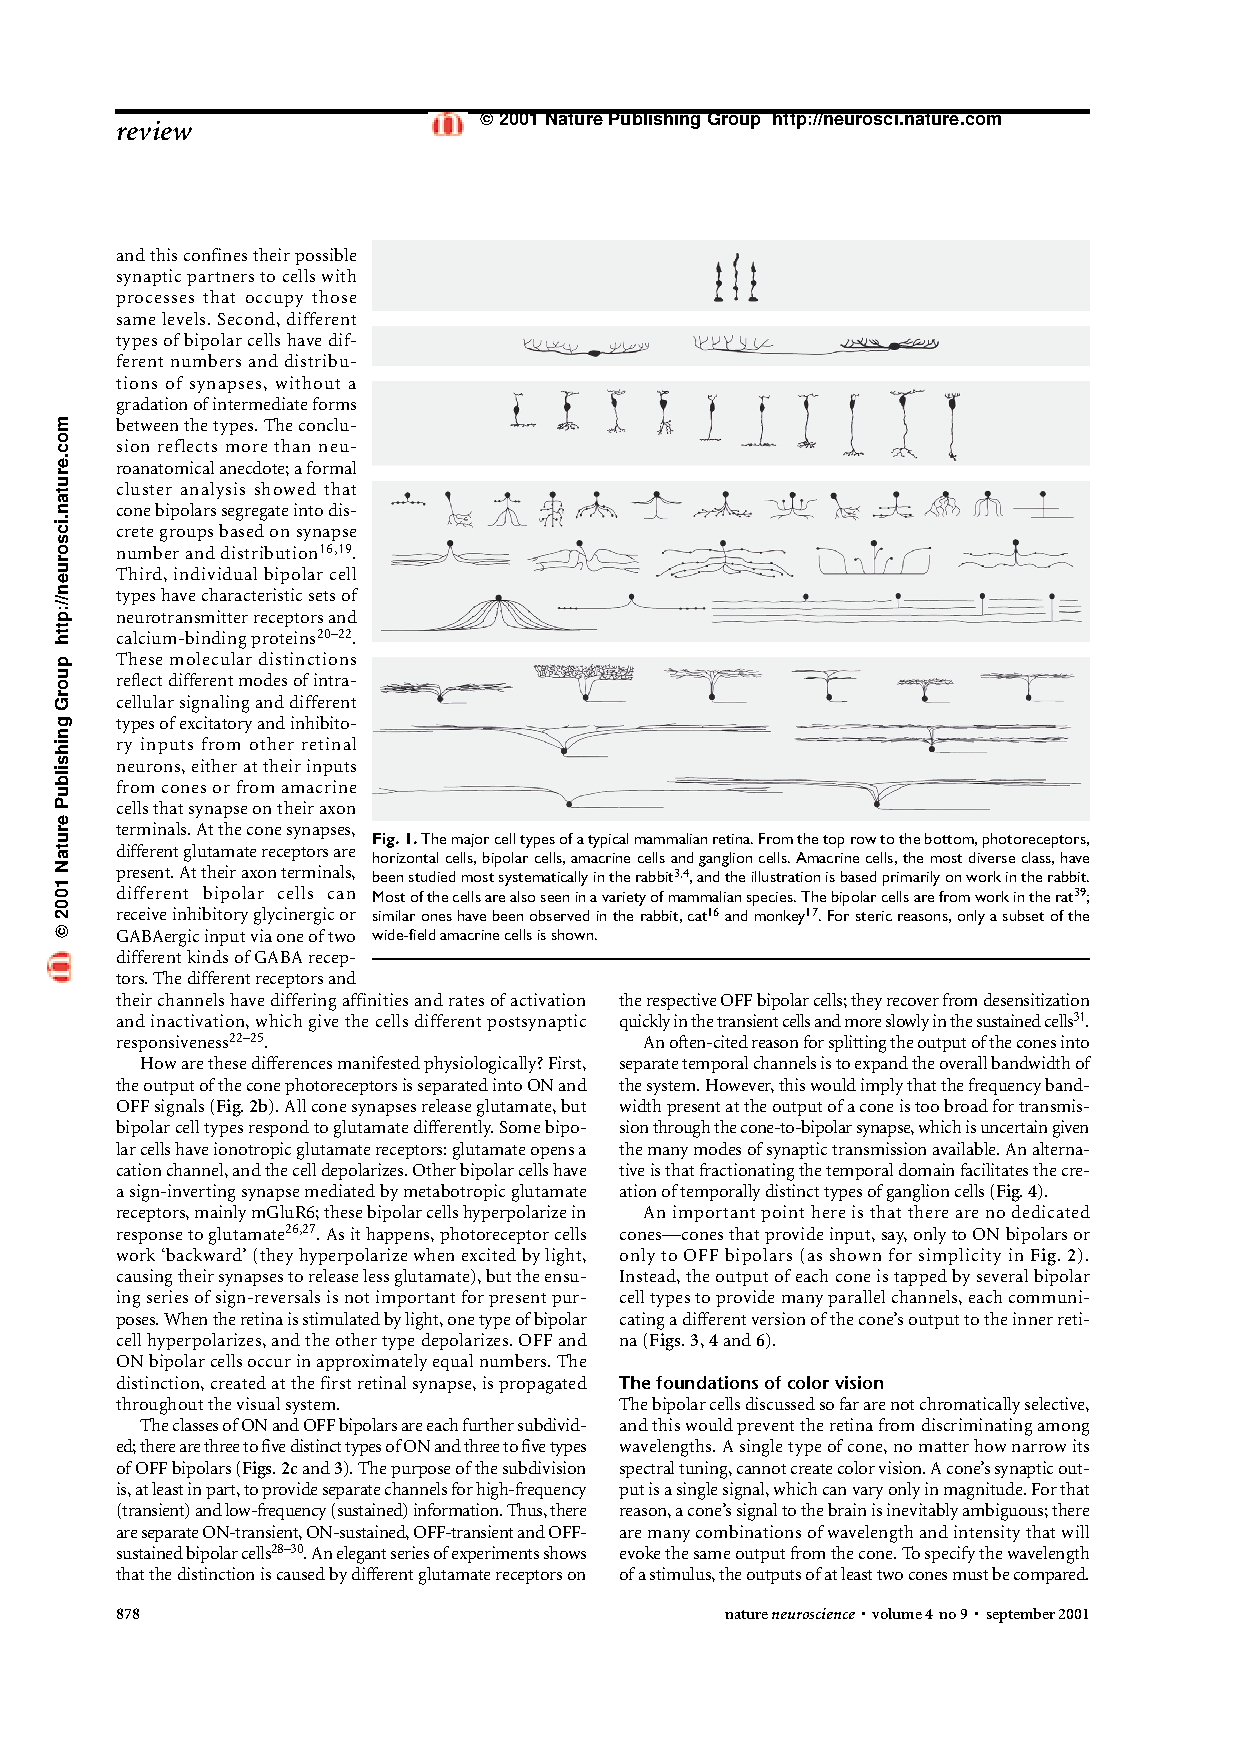
\includegraphics[width=\textwidth, trim=6.2cm 15.7cm 2cm 4cm, clip]{images/masland-2001-neuron-types.pdf}
			\caption{Different types of neuroes in the layers of the retina (from top): photo receptors, horizontal cells, bipolar cells, amacrine cells and ganglion cells \citep{masland2001fundamental}}
		\end{figure}
		
	\section{Optic Chiasm and Lateral Geniculate Nucleus}
	
		In the optic chiasm the signals on the optic nerve are separated into the left and right half frame of the eye. Then the same side signals from both eyes are sent together to the lateral geniculate nucleus (LGN).

		\begin{figure}[H]
			\centering
			\captionsetup{justification=centering,margin=1cm}
			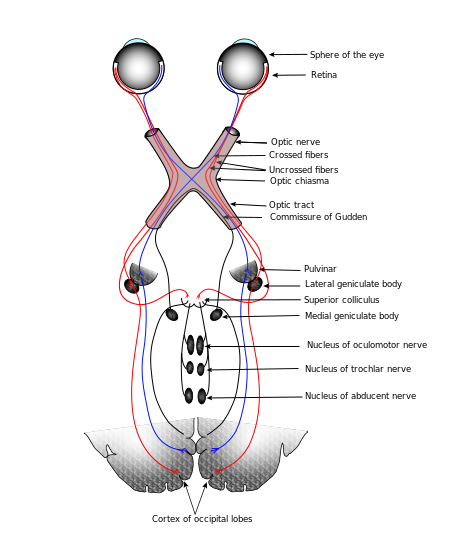
\includegraphics[width=0.7\textwidth]{images/optic-chiasm.png}
			\caption{Overview of the signal flow from the eyes (top) to the visual cortex (bottom), blue lines indicate the nasal side of retinal signals, red the temporal ones}
		\end{figure}

		The major processes that happen in the LGN have to do with combining the signals from the left and right eye. This has little effect on the ability to recognize objects simply because this also works with only one eye.
		
	\section{Visual Cortex} \label{visual-cortex}
	
		The human visual cortex is the biggest single part of the brain. This emphasizes the major role vision has for humans. In about 20 distinct areas the incoming signals from the retina are processed in a mostly hierarchically manner.
		
		Many different regions were identified to perform distinct tasks. Figure \ref{cortex-map} is an example of a map of the connections between these areas. Most of them are bidirectional.

		\begin{figure}[H]
			\centering
			\captionsetup{justification=centering,margin=0.5cm}
			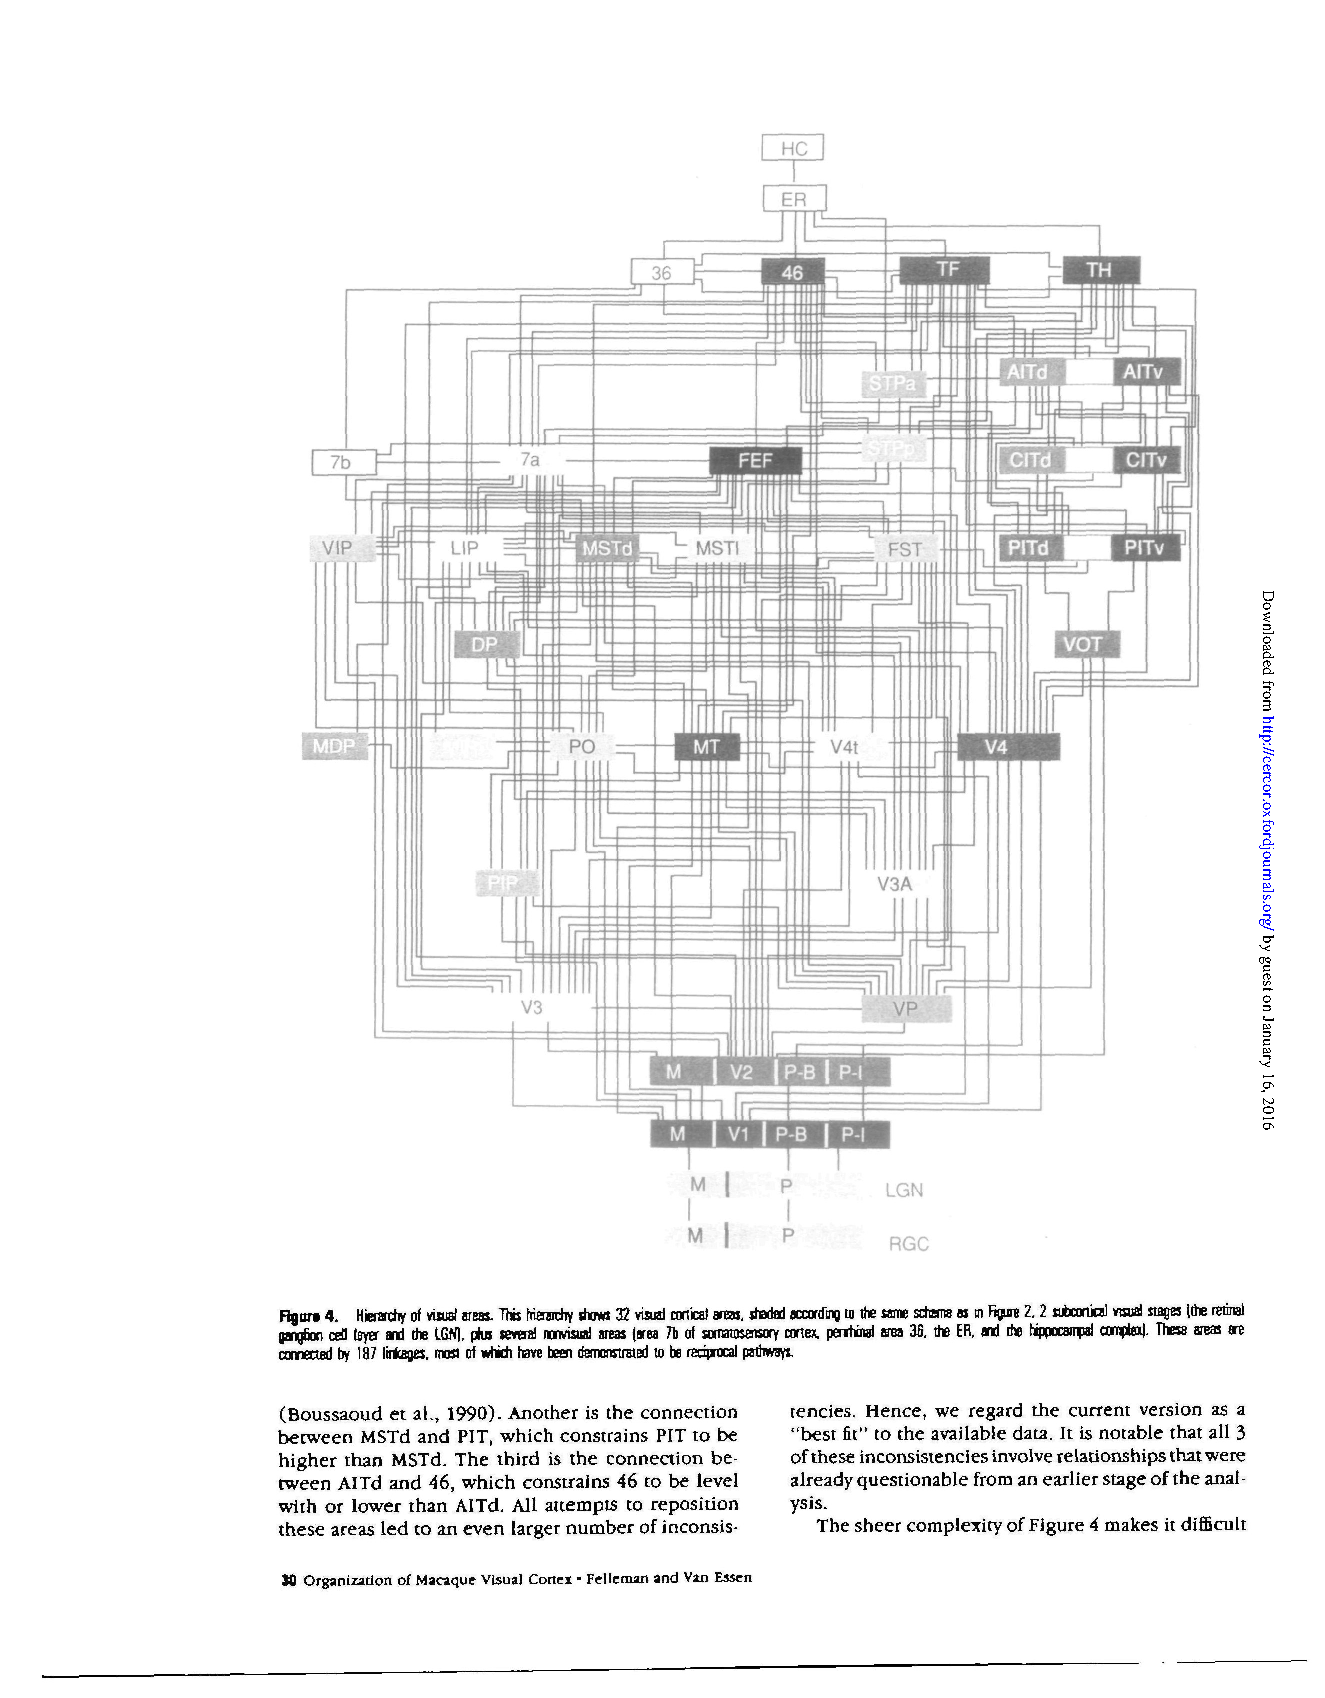
\includegraphics[width=\textwidth, trim=5cm 7cm 2cm 2cm, clip]{images/visual-cortex-map.pdf}
			\caption{Visual cortex map from retina (bottom) to hippocampus (top), most connection are reciprocal \citep{felleman1991distributed}}
			\label{cortex-map}
		\end{figure}
		
		Typically the visual cortex is separated in multiple major areas which are: the primary visual cortex V1 or the striate cortex and the extrastriate areas which are V2 to V5. The information processing is divided into two pathways: The dorsal visual pathway deals with calculating the location of objects meaning a 3D representation and is the connection of the visual cortex with the pariental lobe. The more important one is the ventral visual pathway that conducts the task of what the eyes see and leads to the temporal lobe.
		
		\begin{figure}[H]
			\centering
			\captionsetup{justification=centering,margin=2.3cm}
			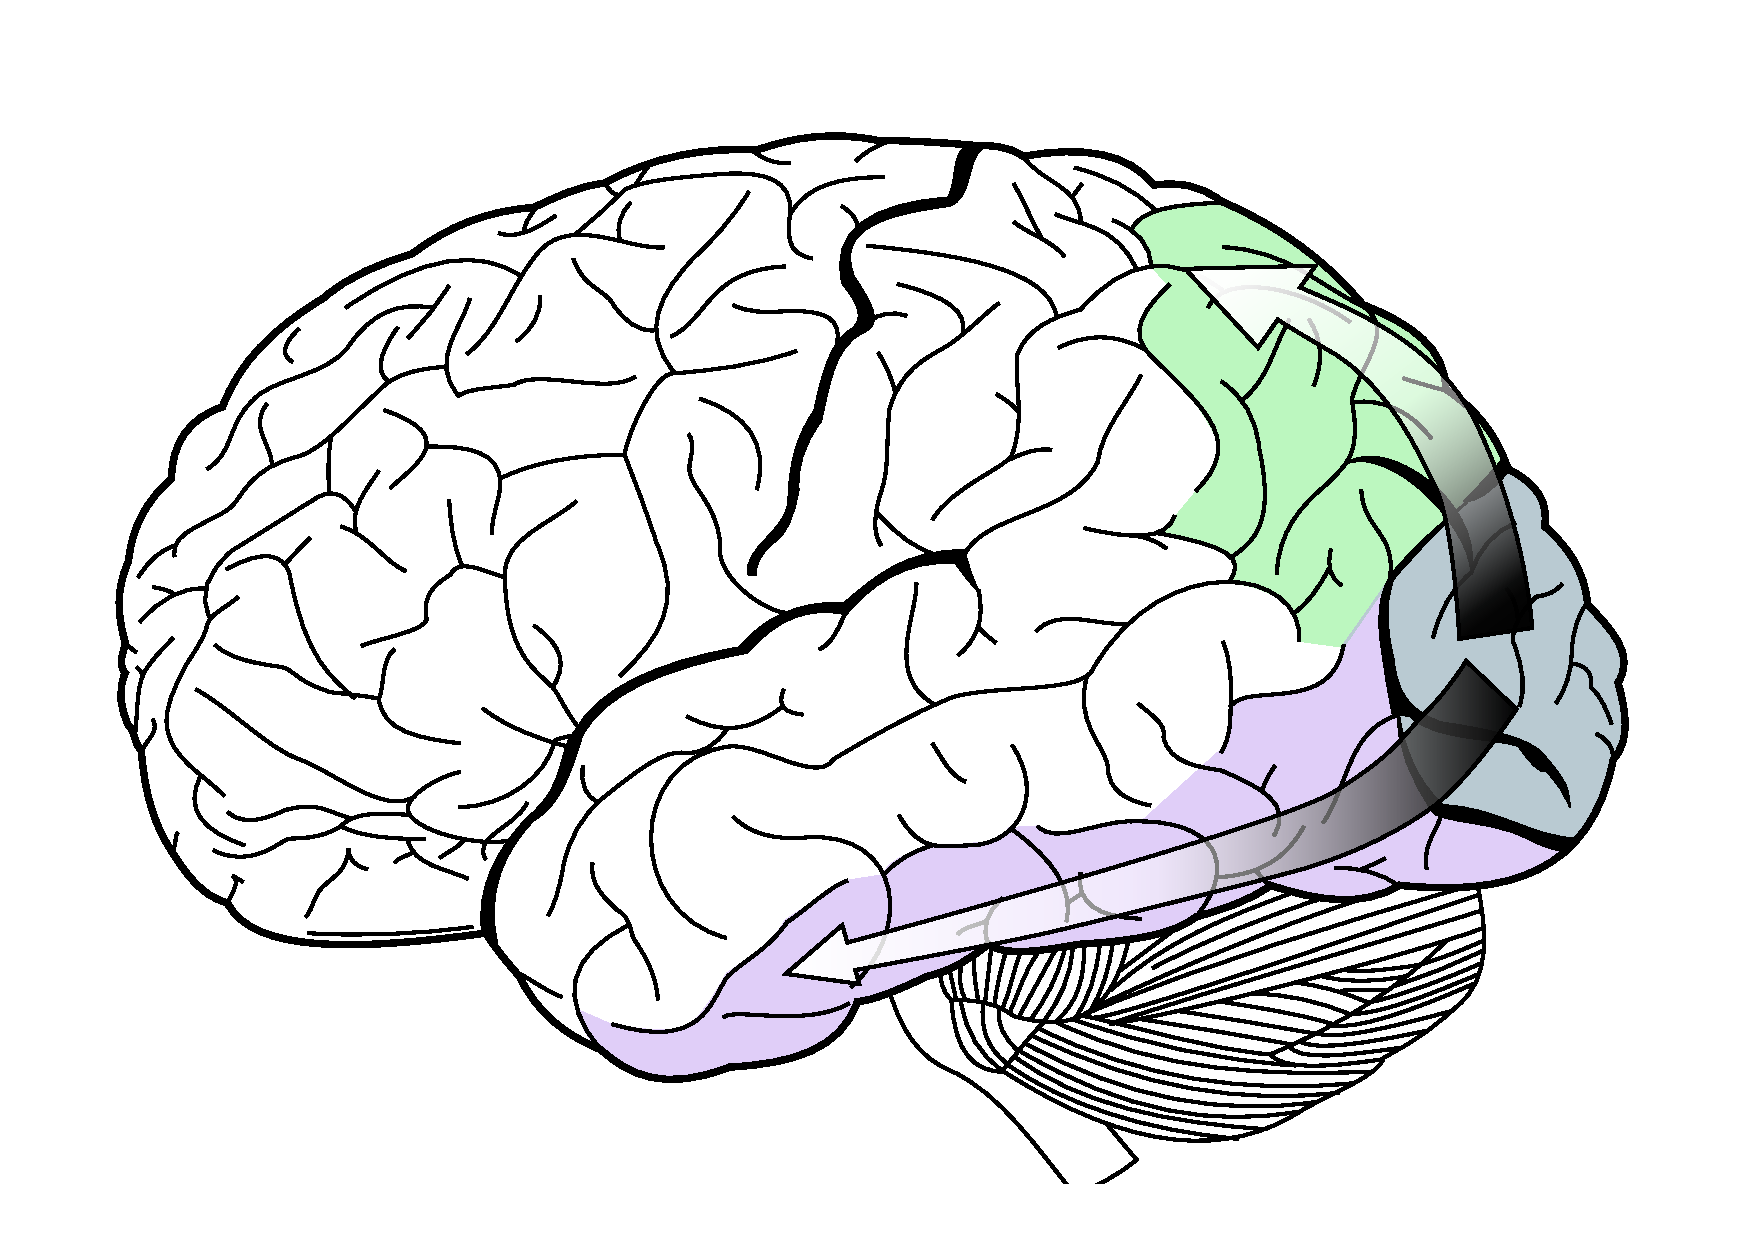
\includegraphics[width=0.7\textwidth]{images/visual-stream2.pdf}
			\caption{Ventral (purple) stream going to temporal lobe and dorsal (green) stream heading to parietal lobe [Source: scholarpedia.org]}
		\end{figure}
		
		In the first layer V1, the primary visual cortex, each neuron only responds to very little areas of the visual field. Basic information about the orientation and movement of objects are obtained. Beginning with the V2 the signals are combined for invariance over the whole visual field. From then on the ventral stream mainly goes along the regions V4 and end in the inferior temporal cortex (IT). In there most of the high-level processing happens. With the connection to the memory areas of the brain, here arise stimuli like recognized objects and faces.
		
		As the information over more and more neurons are combined in higher visual cortex areas, each neuron represents the content of a larger receptive field. At the end invariance of many interferences is achieved, which means an object can be recognized no matter where for example on the input image it is, or what it's rotation is.
		
		A model to explain this was developed by \citeauthor{hubel1962receptive} with the use of so called simple and complex cells. They are described as part of the following chapter.
		
		
\chapter{Biologically Inspired Computational Models of the Visual System}

	Building a model for the visual system will be a compromise. Of course one can start to model every single neuron from the retina to the visual cortex, but this is very unpractical. So the typical step would be to abstract a certain part of the system to a functional description. There are basically two ways to do this: Abstraction top-down and bottom-up.
	
	Top-down means goal-driven, so you could build functional models that abstract viewing tasks, expectations or reasoning. Obviously this is very complicated, therefore bottom-up models, which are stimulus driven, are the way to go.
	
	To realize that kind of model, first of all the signal propagation in the visual system is summed up. Then with the research of \citep{hubel1962receptive} as basis the HMAX model will be explained.

	\section{Basics}
			
		\subsection{Signal Propagation}\label{signal}
			
			The only connection of the retina is the optic nerve. It is about 1 million axons transmitting information in one direction, hence only feed-forward.
			
			Each additional layer of the visual path has back some sort of feedback. As mentioned in chapter 2, almost every connection in figure \ref{cortex-map} is bidirectional. This makes modeling extremely difficult. \citeauthor{thorpe1996speed} found out that even every cortex area of the visual system has some sort of higher function level feedback, in the first 150 milliseconds it is not active. Therefore for this short time one can assume a strict feed-forward network. Despite the fact many features are missing, most models limit themselves to feed-forward.
			
		\subsection{Simple and Complex Cells}
			
			The basis for the following models described in section \ref{hmax} is an achievement by nobel prize winners \citeauthor{hubel1962receptive}. They discovered two types of neurons in the visual cortex: simple and complex cells.
			
			The simple cells respond to light or darkness in a certain area of the visual field, that is called receptive field. They combine multiple ON- of OFF-cells coming from the ganglion layer in the retina as one can see in figure \ref{simple-cell}. Thereby orientation selective simple cells can be modeled.
	
			\begin{figure}[H]
				\centering
				\captionsetup{justification=centering,margin=1cm}
				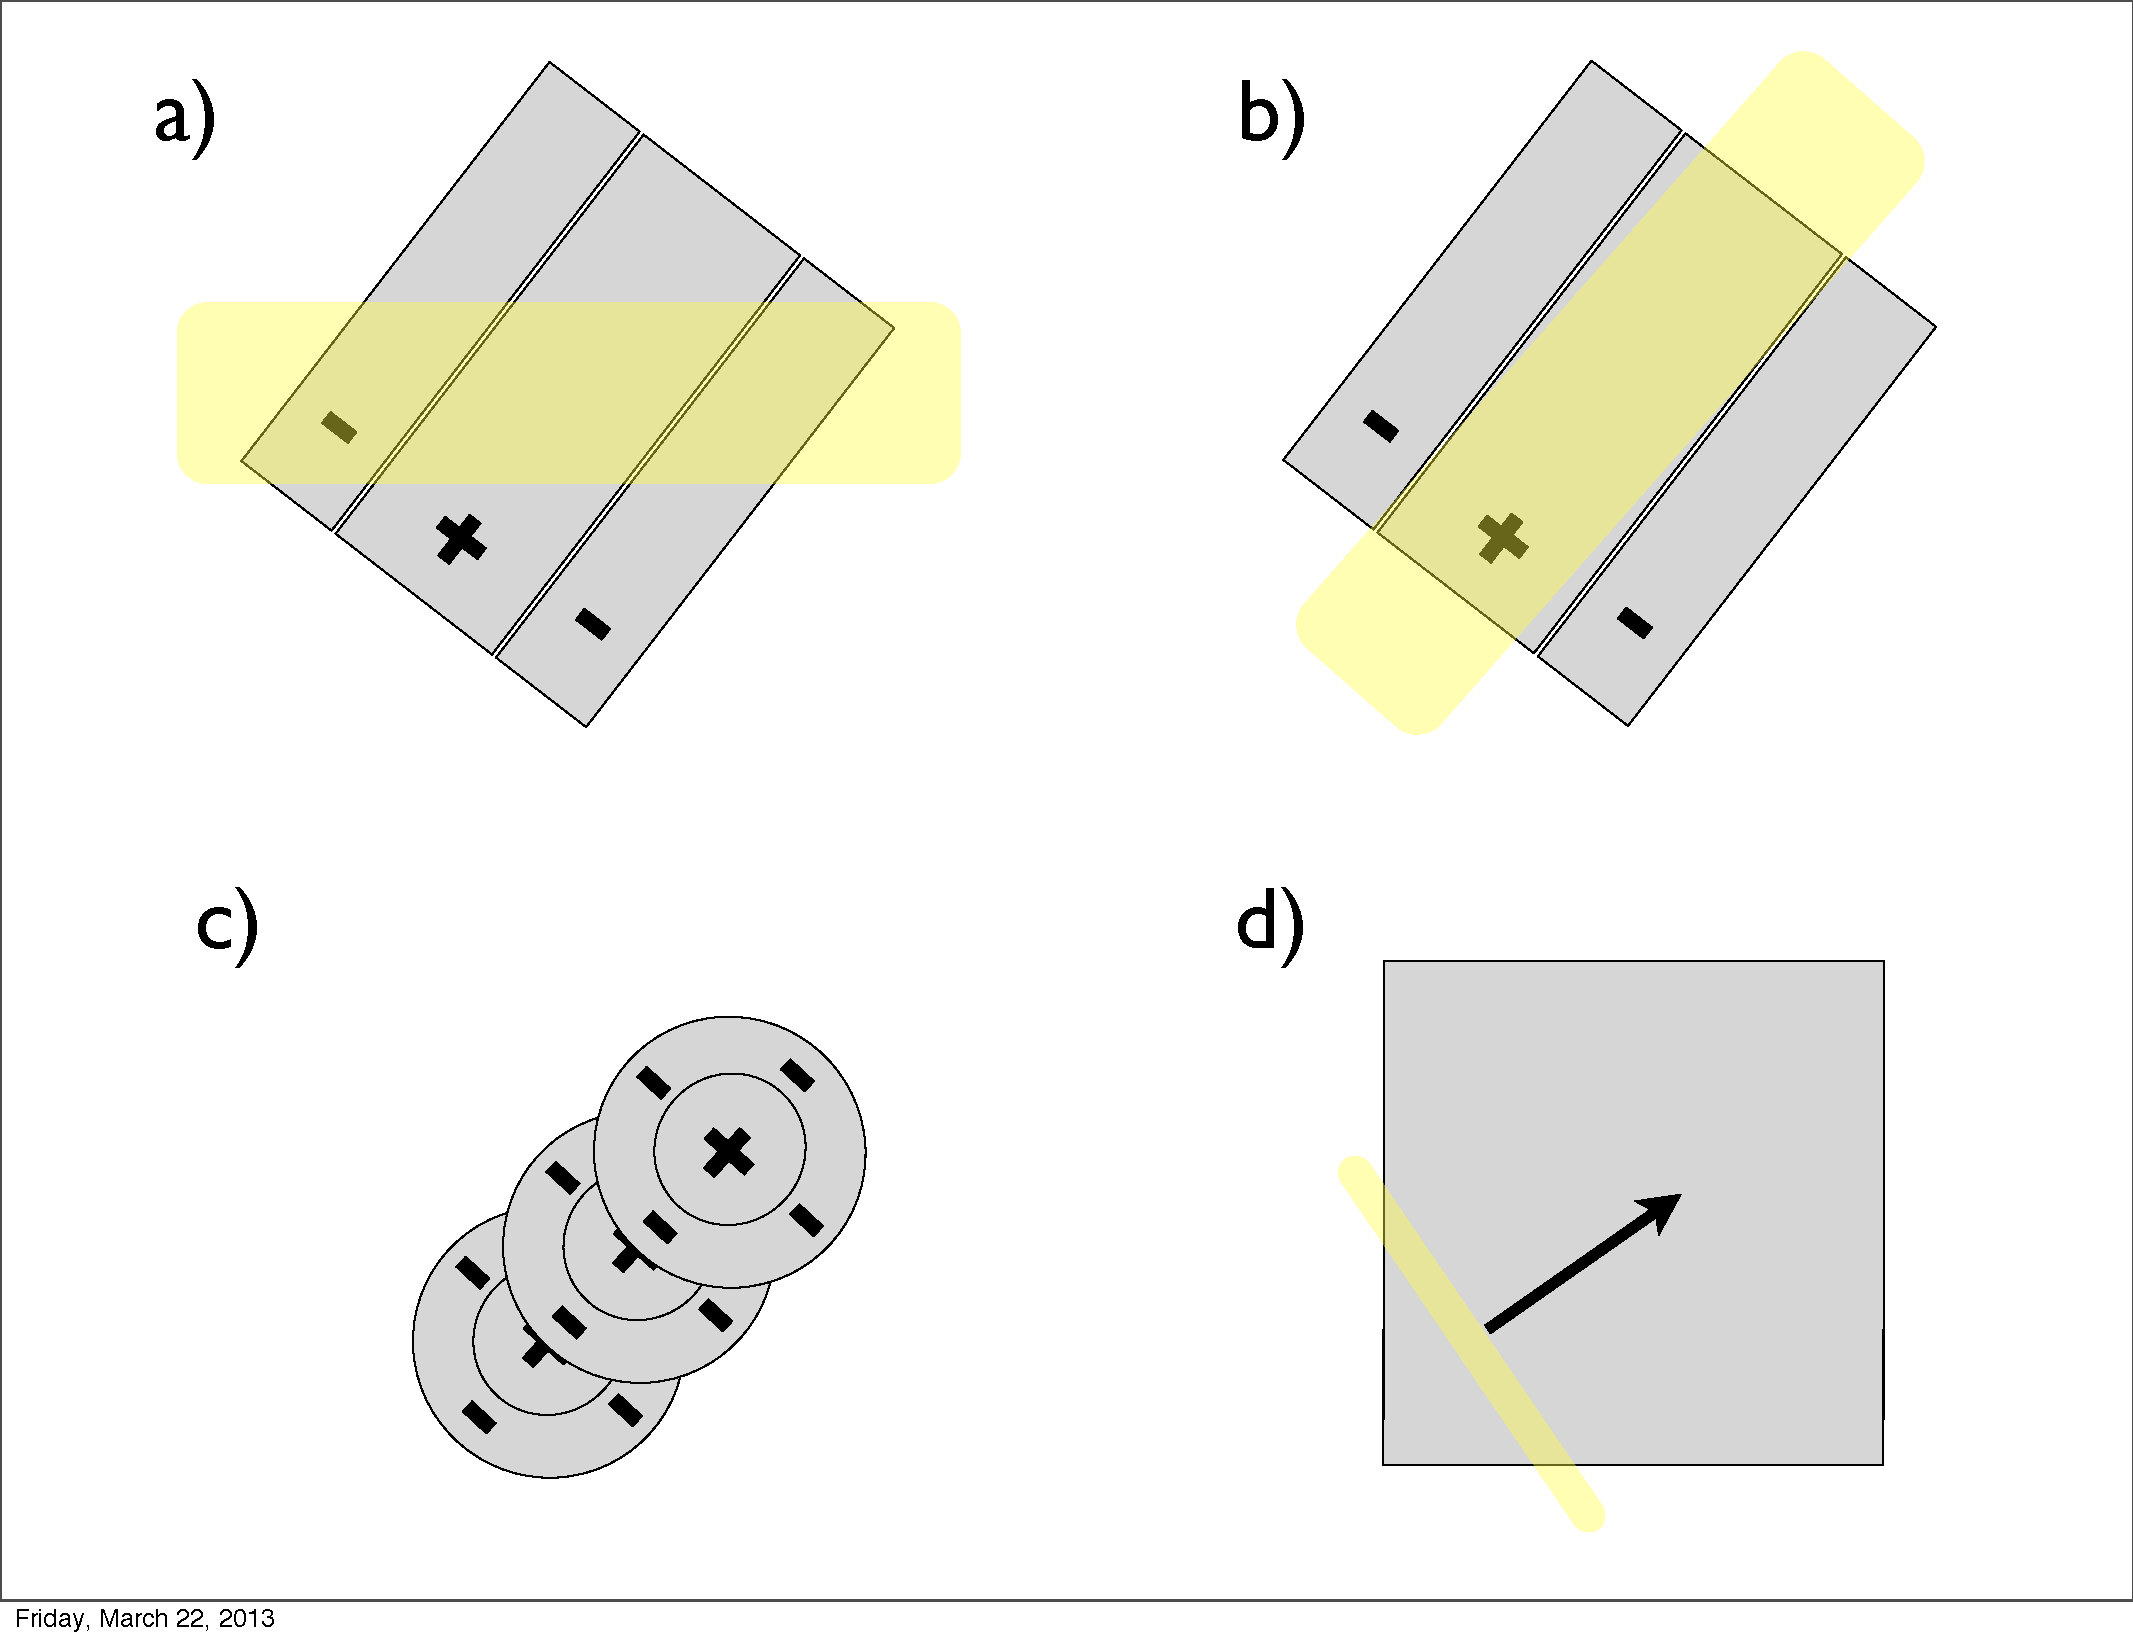
\includegraphics[width=0.2\textwidth, trim=6.9cm 2cm 21.4cm 17cm, clip]{images/Simple_and_Complex_Cells.pdf}
				\caption[https://en.wikipedia.org/wiki/File:Simple\_and\_Complex\_Cells.pdf]{Overlap over multiple ON-center ganglion cells that is performed by a simple cell}
				\label{simple-cell}
			\end{figure}
			
			Complex cells on the other hand combine the output of multiple simple cells and are able to fire when detecting edges or even motion in a specific direction. Figure \ref{hubel-exp} shows a experiment that was performed using a cat as test subject. An electrode was injected into a complex cell in the visual cortex. If the bright white bar was moved in the direction of the drawn arrow, the neuron would fire. If the bar stops or moves the other direction, it would not.
			
			\begin{figure}[H]
				\centering
				\captionsetup{justification=centering,margin=1cm}
				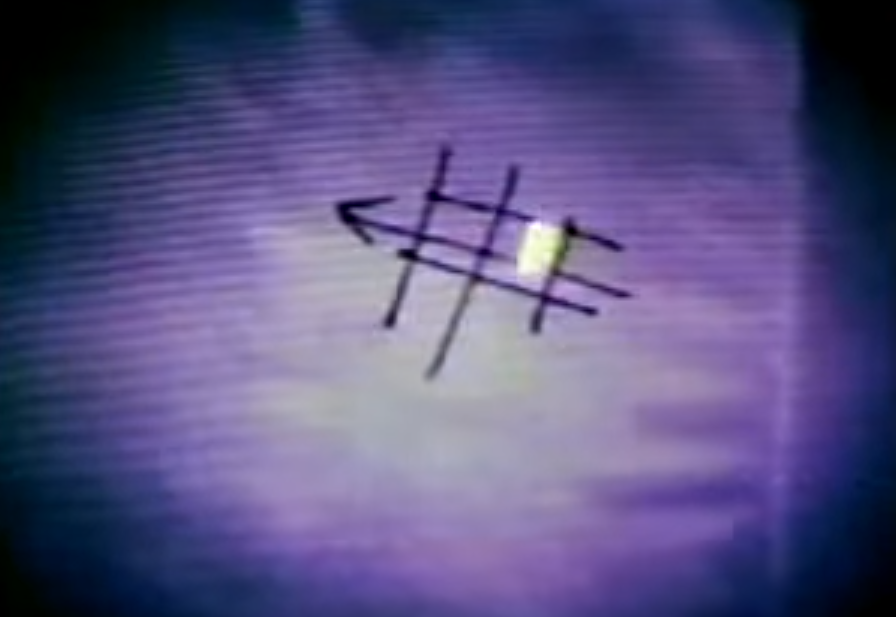
\includegraphics[width=0.5\textwidth]{images/hubel-experiment.png}
				\caption{Experiment performed by \citeauthor{hubel1962receptive}: Complex cell of a cat's visual cortex, the neuron fires only if a short bar is moved in the arrows direction [Source: youtube.com]}
				\label{hubel-exp}
			\end{figure}
			
			In \citep{hubel1965receptive} the two scientists extended their model with the introduction of so called hypercomplex cells. These are basically cells with a complexity beyond the normal complex cells and can be found in higher cortical areas.
			
	\section{Feed-Forward Models}
		
		\subsection{HMAX model for object recognition}\label{hmax}
		
			The research of \citeauthor{hubel1962receptive} was not originally intended for object recognition. It was extended by \citeauthor{riesenhuber1999hierarchical} to form a hierarchical model that uses simple and complex cells as building blocks: the HMAX model. As mentioned in \ref{signal}, as most models this one is strictly feed-forward only. 
		
			\begin{figure}[H]
				\centering
				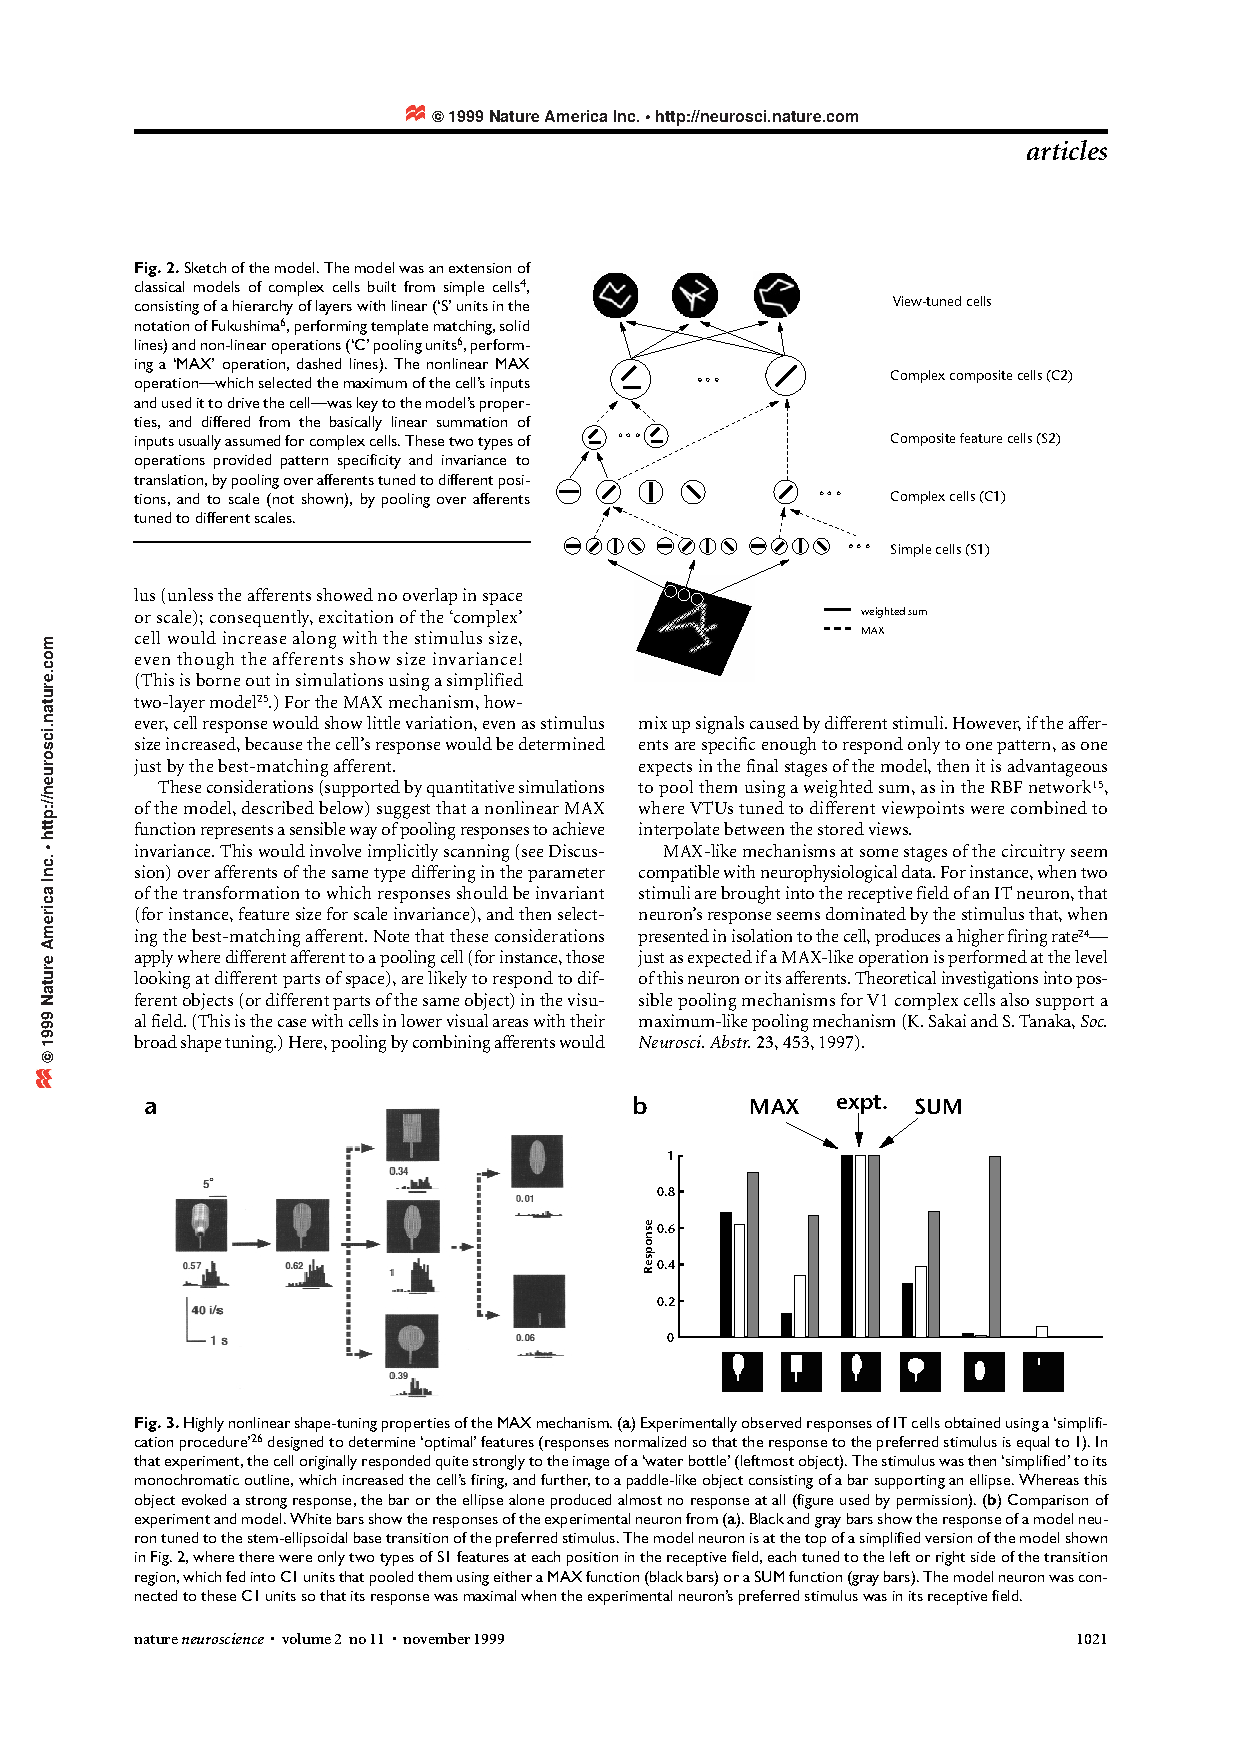
\includegraphics[width=0.8\textwidth, trim= 9cm 18cm 2.5cm 4cm, clip]{images/riesenhuber-poggio-1999-models-p3.pdf}
				\caption{HMAX model by \citep{riesenhuber1999hierarchical}}
				\label{hmax-model}
			\end{figure}
			
			As one can see in figure \ref{hmax-model}, the model consists of 5 layers. The first four layers are alternating simple and complex cells. The first stage features a lattice of blocks that are sensitive to orientation in their respective receptive field. The second layer creates position invariance as it pools over simple cells with the same orientation angle. At S2 these complex cell outputs are composed to selective features such as edges or borders. After another layer that increases invariance over other various transformations, view-tuned cells can describe abstract high-level features like the presence of a specific object. Scale invariance is not shown in this figure, but it is achieved by utilizing different scales of first layer of simple cells and involvement in the subsequent complex pooling operation.
			
			These pooling operations performed by the complex cells are implemented using a nonlinear maximum. This tends to be better than the summation as alternative because it disregards clutter and interferences.
			
			For object identification, supervised learning of the HMAX model works like this: An image of the object is inserted into the model. The response of the second complex cell layer (C2) is recorded and turned into an appropriate view-tuned cell. But there is a need for learning of objects with many pictures differing in perspective, illuminance, position and other transformations. This easily leads to a vast amount of example images for one object.
			
			The two main problems when developing a model for the visual cortex are resolved pretty good. HMAX can provide a high level of invariance in scale, position, rotation and other transformation of the object by simply pooling over the respective cell outputs. Also the selectivity is very high because even on higher layers very sharp edge and border information is used.
			
			\paragraph{Performance} Tests showed that the HMAX model performs very good with natural image sets like Caltech101. But \citep{pinto2008real} argues these images are not at all representative for the task, this model was developed. They feature objects from many different viewing angles in various lightning conditions which is good. This is also stated by the Caltech101 website: "Most images have little or no clutter. The objects tend to be centered in each image."\footnote{\url{http://www.vision.caltech.edu/Image_Datasets/Caltech101}} On real-world image variation, that very well include many interferences, the performance is dropping.
			
			
		\subsection{Extention of HMAX with Template Matching}
		
			A few years later \citeauthor{serre2007robust} extended the HMAX model with template matching functionality which is more closer the biological reality in the inferotemporal cortex \citep{poggio2004generalization}.
			
			The basic assumptions are the same as for the standard HMAX model: the processing is hierarchal (scale and position first, then other transformations), feed-forward processing only and the receptive field is increasing the higher layer a neuron is. But one major thing changes now: Learning is assumed to happen almost at every layer which has to be realized as well as possible.
			
			\begin{figure}[H]
				\centering
				\captionsetup{justification=centering,margin=1cm}
				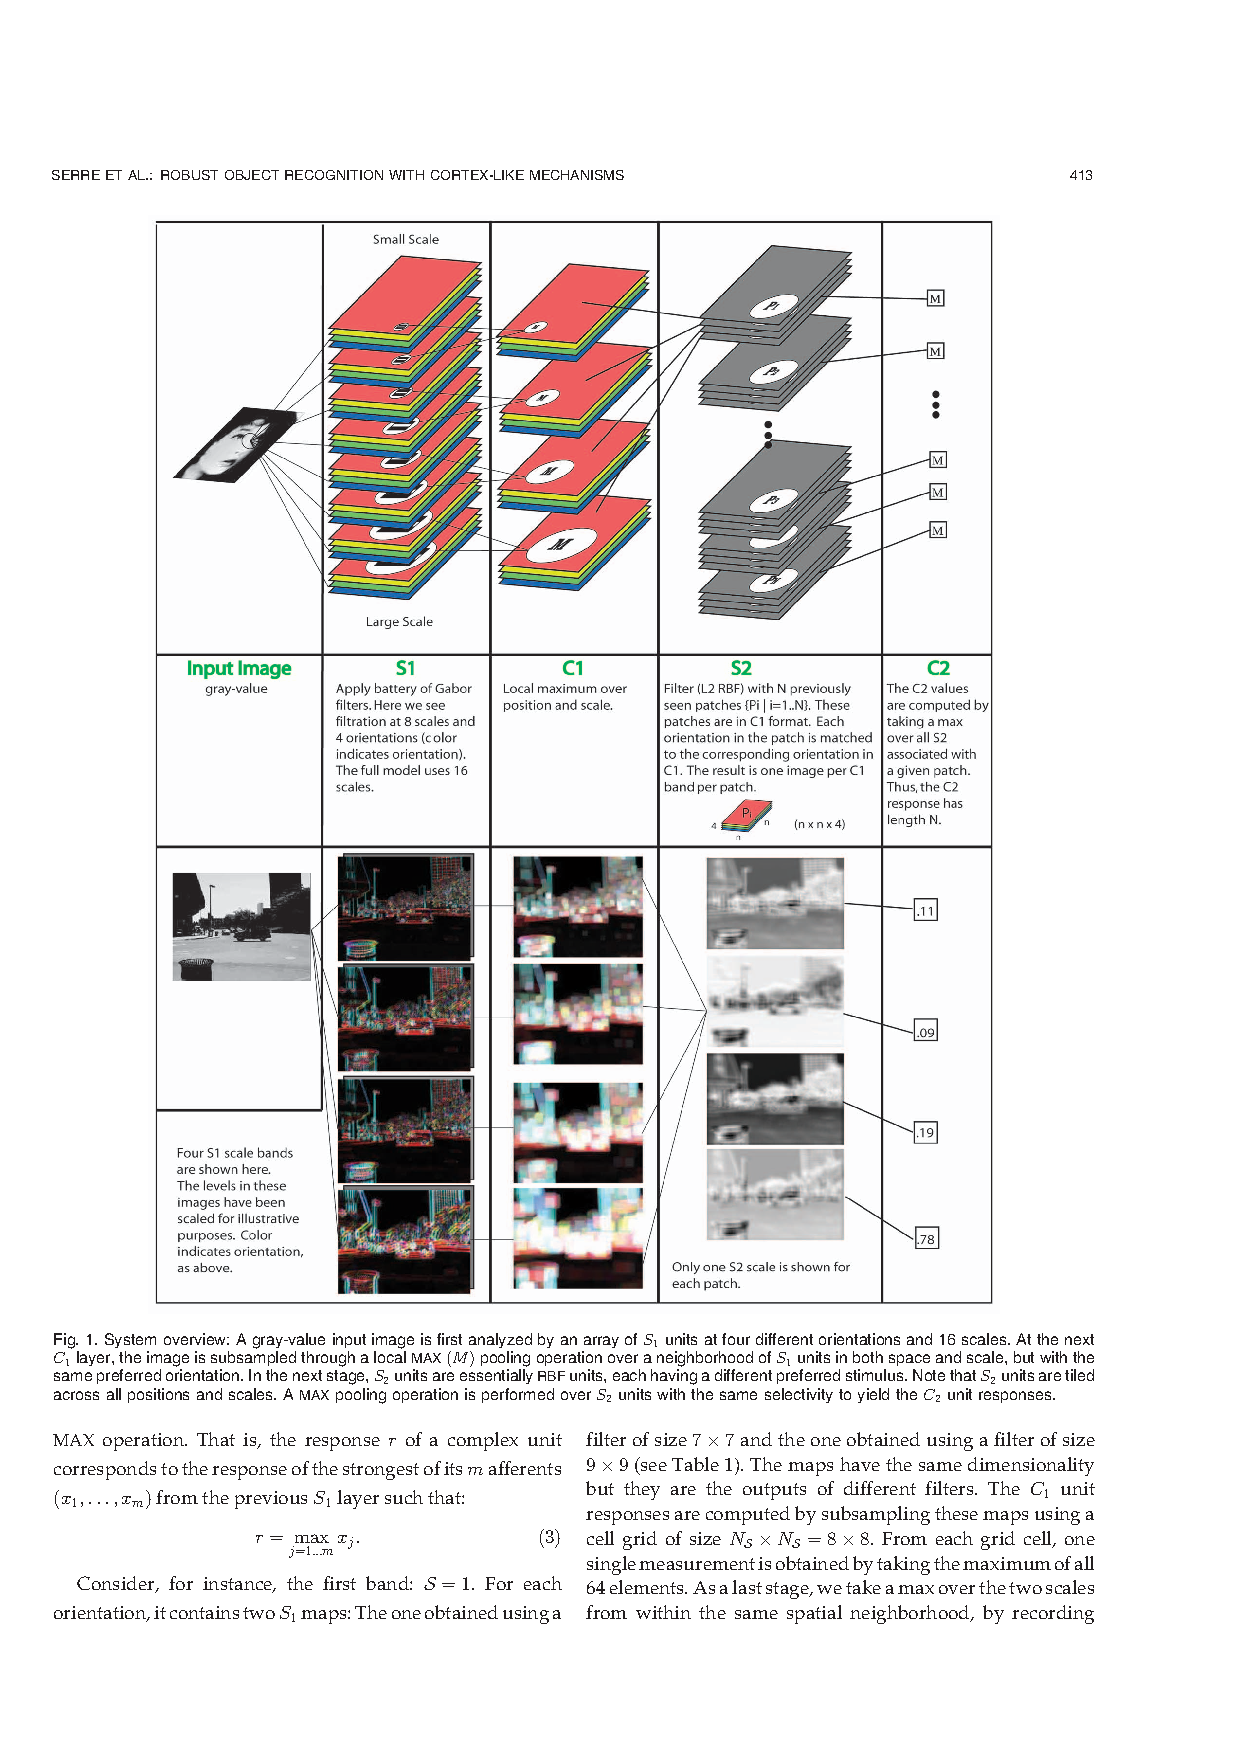
\includegraphics[width=\textwidth, trim= 2.5cm 18.2cm 4cm 3.5cm, clip]{images/serre-appearance-based-model.pdf}					%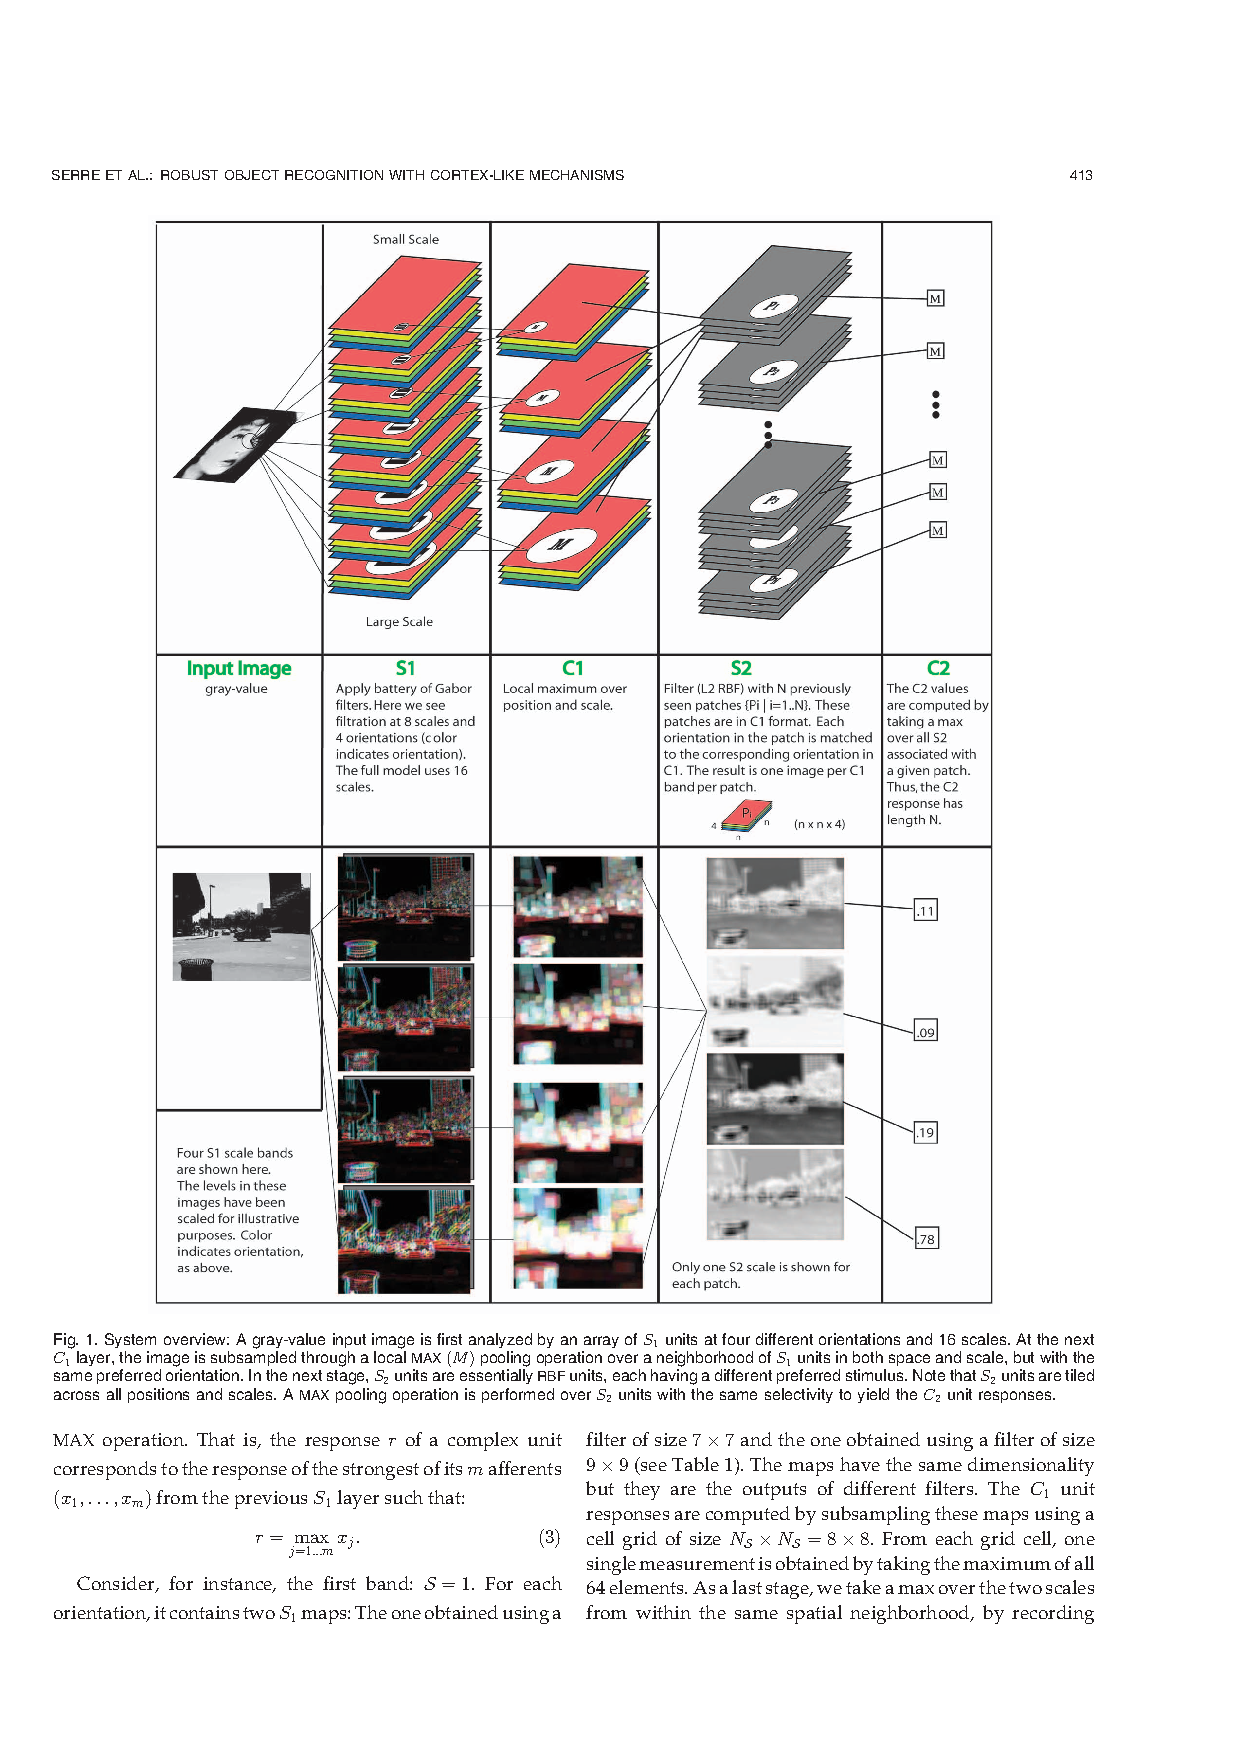
\includegraphics[width=\textwidth, trim= 2.5cm 18.61cm 4cm 3.5cm, clip]{images/serre-appearance-based-model.pdf}				%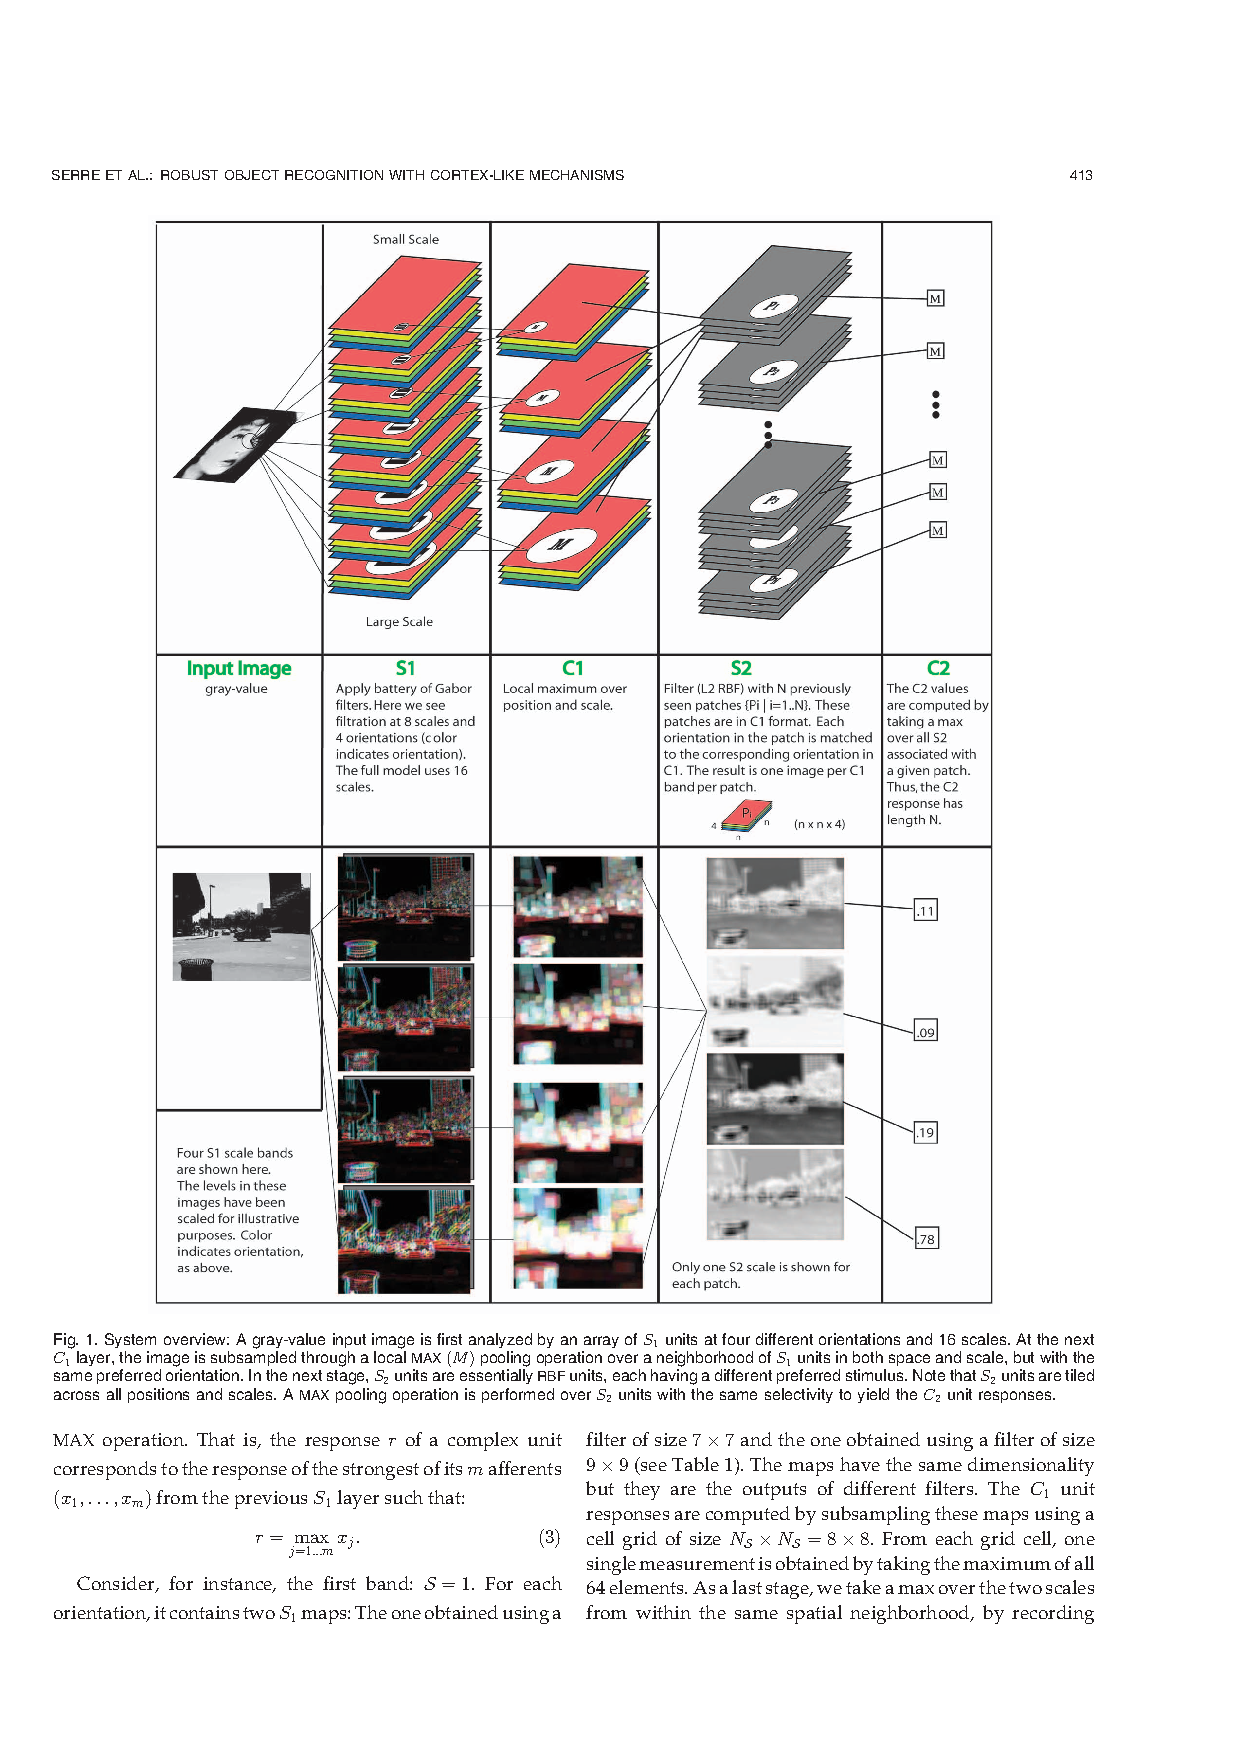
\includegraphics[width=\textwidth, trim= 2.5cm 15.35cm 4cm 3.5cm, clip]{images/serre-appearance-based-model.pdf}
				\caption{System overview of the model (Source: \citep{serre2007robust})}
				\label{serre-model}
			\end{figure}
			
			The figure \ref{serre-model} shows the proposed model with it's four stages. In the first one, $ S_1 $, for an incoming gray-scale image, multiple Gabor filters (16 scales and 4 orientations) are applied:
			
			\begin{align*}
				F\left(x,y\right) = e^{-\frac{x_0^2+\gamma^2 y_0^2}{2 \sigma^2}} \times \cos\left(\frac{2\pi}{\lambda}x_0\right)
			\end{align*}
			
			mit \vspace*{-0.8cm}
			\begin{align*}
			 x_0 &= x \cos\Theta + y \sin\Theta \\
				y_0 &= -x \sin\Theta + y \cos\Theta \\
				\Theta &= 0^\circ; 45^\circ; 90^\circ; 135^\circ
			\end{align*}
			
			\vspace*{0.2cm}
			
			The exact parameters can be looked up in the original paper:  \citep{serre2007robust}.
%			
%			The parameters are the aspect ratio $ \gamma = 0.3 $, the effective width $ \sigma $, the wavelength $ \lambda $ as well as the filter sizes $ s $. All missing values can be seen in figure \ref{serre-model-s1-vals}. These were determined on basis of data by other research groups.
%
%			\begin{figure}[H]
%				\centering
%				\captionsetup{justification=centering,margin=1cm}
%				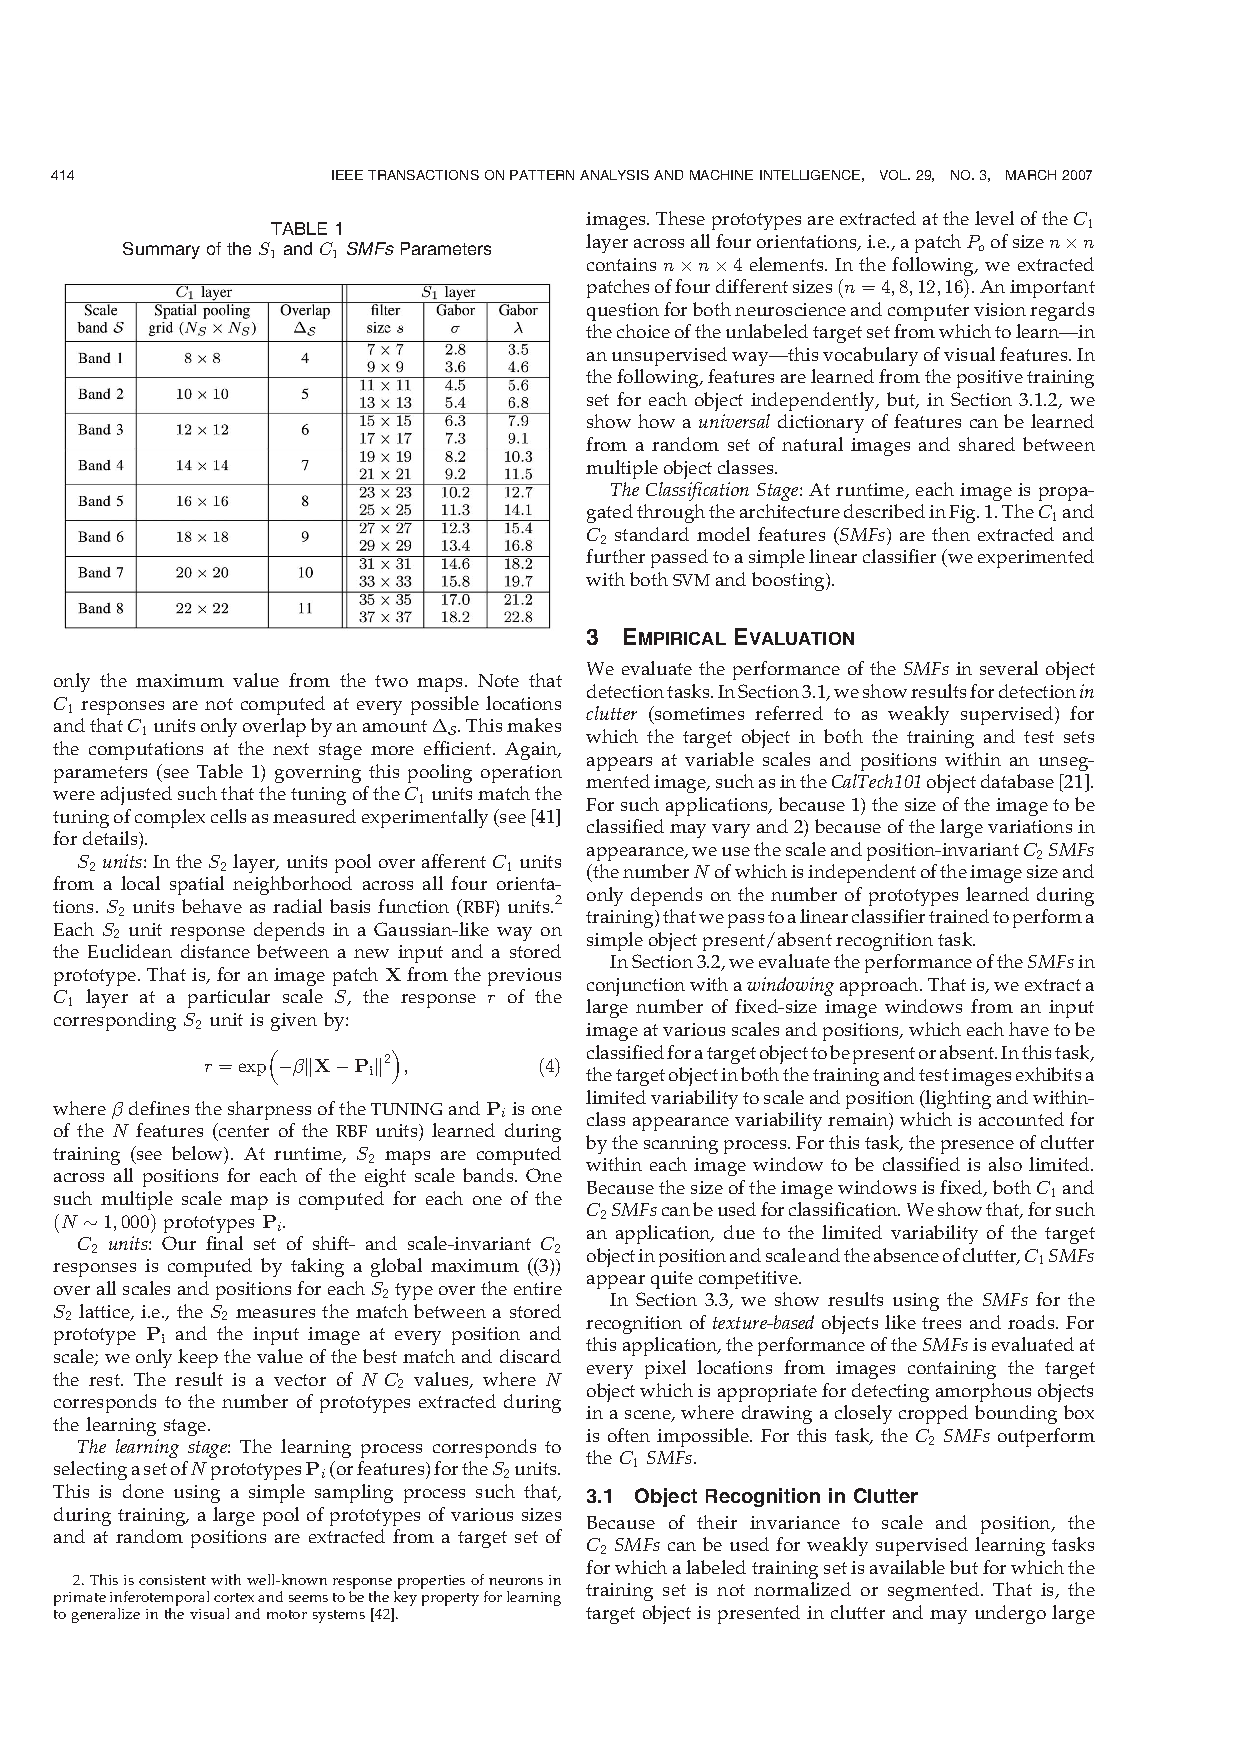
\includegraphics[width=0.5\textwidth, trim=0.5cm 19cm 11.5cm 4.5cm, clip]{images/serre-appearance-based-model2.pdf}	
%				\caption{Parameters for the $ S_1 $ stage of the model calculated with the help of data by other research teams (Source: \citep{serre2007robust})}
%				\label{serre-model-s1-vals}
%			\end{figure}
%			

			\vspace*{0.3cm}

			These filters create 64 different output images. In the next stage, $ C_1 $, the complex cells provides the local maximum over position, thus providing shift invariance. During this operation always two of the 16 scales are combined, leaving a total of 32 images (8 sets with 4 different filter orientations).
			
			These are compared with a vast amount of trained feature patches in $S_2$. This is the template matching that is new to the model. The determination of the training patches is simple: A target set of pictures of objects that should be recognized is acting as input of the model. The feature values are then simply taken from the $C_1$ output. Later every new image will be compared to all available trained feature values with a radial bias function (RBF):
			
			\[ r = e^{-\beta \vert\vert \textbf{X} - \textbf{P}_i \vert\vert^2 } \]
			
			The higher the value $ r $, the better the correspondence to the trained feature.
			
			$C_2$ finally pools over all $S_2$ outputs of the same feature patch and saves only the maximum. This leaves a vector with the length of the trained patches.
			
			\paragraph{Performance} A major limitation could be the $S_1$ and $C_1$ stages that do need much computational effort. But the overall performance shown in , especially in comparison with SIFT, proves it being worth it (see figure \ref{serre-performance}).
			
			\begin{figure}[H]
				\centering
				\captionsetup{justification=centering,margin=1cm}
				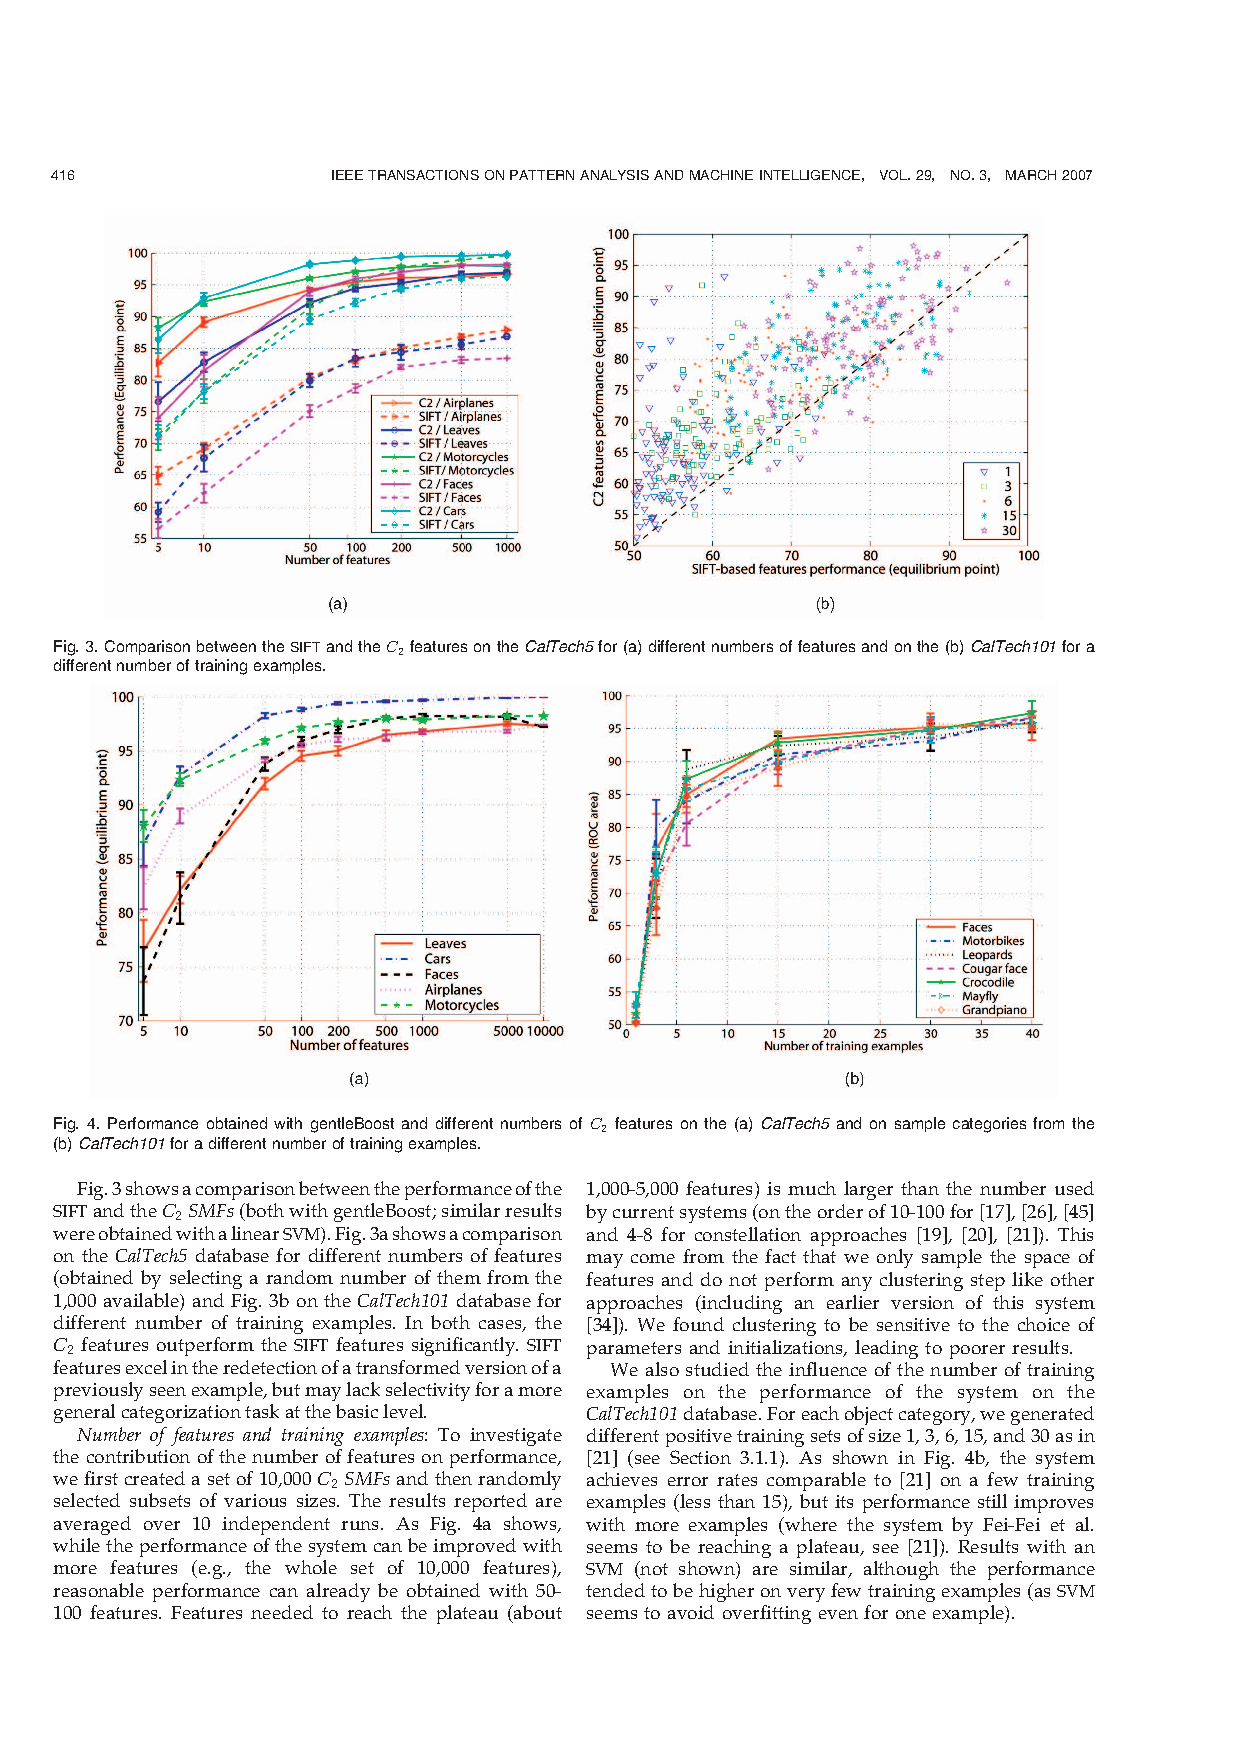
\includegraphics[width=0.5\textwidth, trim=1.8cm 20cm 12cm 4cm, clip]{images/serre-appearance-based-model3.pdf}
				\caption{Performance of model proposed by \citep{serre2007robust}}
				\label{serre-performance}
			\end{figure}
			
			All performance tests in the paper were conducted while not tuning one single parameter. These were determined using data about the primary visual cortex. Improvements are very well possible.
			
			As opposed to having a broad categorization performance, specializing on object identification is way easier. Reference images have to be learned as explained above. In the process of recognition, the radial basis function will provide a high value just because it is not a feature but more like a specific object patch.

	\section{Biological plausibility}
	
		\paragraph{Simple and Complex Cells} Many parts of the HMAX model were designed with the experiments of \citeauthor{hubel1962receptive} in mind. These only represent a very basic computational part in the visual cortex. Nevertheless it is necessary, that it is possible to realize the two main building blocks of the model, the simple and complex cells, in neuronal circuits. If that would not be possible, further investigations would be pointless. This was studied in \citep{serre2005theory} with a positive result.
		
		\paragraph{No Feedback} One of the main problems the presented models have is the strict limitation to feed-forward networks. As outlined in section \ref{visual-cortex}, this is absolutely not true. There are several attempts to achieve this but they mostly have major deficits. This is understandable when looking at a functional map of the visual cortex (figure \ref{cortex-map}). The connections reach up to the hippocampus and are influenced by cognitive behavior. Also it is arguable if integration of higher brain functions will lead to better object recognition performance.
		
		\paragraph{Learning} While making it possible to reduce the amount of images needed for training of object recognition models, humans still are way better. They normally can recognize an object with only one single example as trained reference.
		
\chapter{Application: Localization}

	One of many possible applications for object recognition in general is self-localization. Therefore stationary objects, called landmarks, have to be recognized and associated with position information.
	
	A simple example: A robot drives through a hallway. There are many different object to recognize that he knows, like a door. But usually there is not only a single door but many different. If recognizing more objects in the surrounding area, like windows, plants or hallway junctions, the possible locations for this kind of specific occurrences is limited. This is normally implemented using a particle filter that is for example explained in \citep{siagian2009biologically}.
	
	But what requirements does this have for the object recognition algorithm? First of all the computational effort should be kept within reasonable limits. Normally the self-localization is not the primary task when there is the need for it. Secondly the image of the camera does not focus automatically onto specific separated objects. There will always be much clutter in the model inputs. One way to overcome this issue is more extensive training. But this is in conflict with the third requirement for object recognition algorithms: Ideally it does not need much object examples to perform well. It is highly unpractical if for indoor navigation every object in each single room has to be trained with hundreds of images.
	
	
\chapter{Conclusion}

	
	models must be extended using more layers (S3, C3)
	
	doubtful if current feedback research will improve object recognition performance
	
	
	
	